\documentclass{article}
\usepackage[utf8]{inputenc}

\newenvironment{changemargin}[2]{%
\begin{list}{}{%
\setlength{\topsep}{0pt}%
\setlength{\leftmargin}{#1}%
\setlength{\rightmargin}{#2}%
\setlength{\listparindent}{\parindent}%
\setlength{\itemindent}{\parindent}%
\setlength{\parsep}{\parskip}%
}%
\item[]}{\end{list}}

\usepackage{geometry}
\newgeometry{left=3cm,top=2cm}

\usepackage[pdftex]{hyperref}
\usepackage{graphicx,float}
\usepackage{parskip}
\usepackage{caption}
\usepackage{amsmath}
\usepackage{listings}
\usepackage{xcolor}
\lstset { %
    language=Python,
    backgroundcolor=\color{black!5}, % set backgroundcolor
    basicstyle=\footnotesize,% basic font setting
}


\title{\textbf{Artigo - Modelagem de Fenômenos Biológicos}}
\author{\textbf{Raphael Levy e Erick Brito}}
\date{}

\begin{document}

\maketitle
\\
\begin{center}
    \textbf{\Large{Resumo}}
    \\\\Nesse artigo iremos analisar o comportamento dinâmico de um quimiostato baseado em um modelo com equação de Monod, um tipo de modelo para o crescimento de microrganismos desenvolvido por Jacques Monod.
\end{center}
\\\\
\begin{center}
    \textbf{\Large{Abstract}}
    \\\\In this article we will analyze the dynamic behavior of a chemostat based on a model with Monod equation, a type of model for the growth of microorganisms developed by Jacques Monod. 
\end{center}
\\\\
\\
\textbf{\Large{Introdução}}
\\\\Como forma de avaliação para o curso de Modelagem de Fenômenos Biológicos, decidimos analisar modelos de crescimento de microrganismos. Mais precisamente, escolhemos analisar o modelo de um \textbf{quimiostato} ($\textbf{chemostat}$, em inglês). O quimiostato é um tipo de biorreator, um equipamento laboratorial inventado em 1950 quase que simultaneamente por Jacques Monod e Aaron Novick $\&$ Leo Szilard, em que um meio de cultura ``fresco" (substrato) é continuamente adicionado, enquanto que o meio anterior com o substrato ``restante" é continuamente removido na mesma taxa, mantendo o volume constante, e é usado para controlar a taxa de crescimento dos microganismos presentes $^{[1]}$. Além disso, é possível também regular níveis de pH, temperatura e oxigenação $^{[2]}$. O nome em si significa ``[ambiente] químico estático".

\begin{figure}[H]
        \centering
        \hbox{\hspace{7.0em} 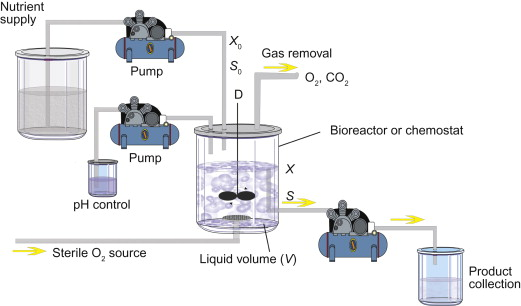
\includegraphics[scale=1.0] {Funcionamento_Quimiostato.jpg}} 
        \caption*{Funcionamento de um quimiostato $^{[2]}$}
\end{figure}
\\\\Um exemplo de funcionamento de um quimiostato pode ser encontrado em $^{[4]}$.
\\\\Para análise de competições entre organismos no quimiostato, são utilizados modelos matemáticos baseados em equações diferenciais, com algumas pequenas variações dependendo do estudo feito. Originalmente, muitos modelos de quimiostato assumiam que o coeficiente de rendimento de biomassa era constante, mas observações experimentais indicavam que um rendimento constante não poderia explicar o comportamento oscilatório presente no quimiostato, como indicado por Rana e Kulsum $^{[5]}$, o que ocorre, em particular, com células de $Saccharomyces cervisae$ e de fitoplâncton $^{[6]}$, organismos estudados por Porro $et \ al.$, que estudavam a aparição espontânea de oscilações em condições aeróbicas em culturas de levedura $^{[7]}$, e por Nisbet e Gurney, que estudavam a resposta de populações a flutuações ambientais contínuas $^{[8]}$. 
\\\\Foi sugerido então que se usasse um coeficiente linear, com um ciclo limitante, e posteriormente Huang $^{[9]}$ e Pilyugin e Waltman $^{[10]}$ desenvolveram modelos com um rendimento variável em vários ciclos, porém esses modelos ainda consideravam apenas o estudo de um único microrganismo por vez. Assim, em 1999, um modelo tridimensional, desenvolvido por Song G. e X. Li $^{[11]}$, que utilizava dois microrganismos, com funções de reações de tipo Monod \footnote{Uma equação Monod é um tipo de modelo matemático para o crescimento de microrganismos, desenvolvido por Monod, relacionando a taxa de crescimento dos microrganismos com a concentração de meio nutritivo limitado em um ambiente aquoso. A equação é dada por:
\begin{center}
    $\mu = \mu_{max} \frac{[S]}{K_s + [S]}$
\end{center}
Onde $\mu$ é a taxa de crescimento do microrganismo em estudo, $\mu_{max}$ é a taxa máxima de seu crescimento, $[S]$ é a concentração do substrato limitante para o crescimento $S$ e $K_s$ é o valor de $[S]$ quando $ \mu/\mu_{max} = 0.5$ ($K_s$ é a ``constante da meia-velocidade").\\\\} $^{[12]}$ e coeficientes de rendimento assumidos como uma função linear da concentração de nutriente, conseguiu estabilidade.
\\\\Em contrapartida, outros estudos indicam que a taxa de crescimento não se ajusta de forma imediata às mudanças no estado estacionário da entrada de substrato ou na taxa de diluição, como previsto por uma equação de Monod, mas na verdade passa por um ``atraso" em resposta às alterações na cultura, que é conhecido como um fenômeno inerte ou efeito de histerese \footnote{Tendência de um sistema de conservar suas propriedades na ausência de um estímulo que as gerou $^{[14]}$, retardo de um efeito quando forças agindo sobre o corpo ou sistema são alteradas $^{[15]}$.}. Assim, foram desenvolvidos modelos que levam em consideração uma equação dinâmica que relaciona a taxa de crescimento específica à concentração de substrato limitante no quimiostato $^{[13]}$. Nesse artigo íamos estudar o modelo dinâmico proposto por Young $et \ al.$, porém como esse modelo faz uso de quações com atraso, decidimos modelar as análises usando o modelo ``simples" de Monod. As equações abaixo vieram ambas dos estudos de  Young $et \ al. $ $^{[13]}$ 
\\\\
\textbf{\Large{Metodologia}}
\\\\O modelo que utilizaremos será o modelo de Monod:
\begin{align}
    (dX/dt) &= \mu X-DX     
  \\(dS/dt) &= DS_0-DS-(\mu X/Y)
  \\\mu &= \hat{\mu}(S/(K_s+S))
\end{align}
\\\\Onde:

\begin{itemize}
\item $X$ = Concentração de massa celular (Massa/Volume)
\item $S$ = Limite de concentração de saída do substrato (Massa/Volume)
\item $S_o$ = Limite de concentração de entrada do substrato (Massa/Volume)
\item $D$ = Taxa de diluição (1/Tempo)
\item $\mu$ = Taxa de crescimento específica (1/Tempo)
\item $\hat{\mu}$ = Máxima taxa de crescimento específica (1/Tempo)
\item $Y$ = Coeficiente de rendimento (Massa celular/Massa do substrato limitante)
\item $K_s$ = Constante de saturação (Massa/Volume)
\end{itemize}
\\\\Analisando as equações (1), (2) e (3) dimensionalmente temos:
\begin{itemize}
    \item A taxa $\frac{dX}{dt}$ do lado esquerdo de (1) tem as unidades $\frac{Massa/Volume}{Tempo} = \frac{Massa}{Volume \cdot Tempo}$. Observando o lado direito, $\mu X - DX$, e substituindo pelas unidades teremos: 
    $$\frac{Massa}{Volume} \cdot \frac{1}{Tempo} - \frac{1}{Tempo} \cdot \frac{Massa}{Volume}$$
    $$= \frac{Massa}{Tempo \cdot Volume}$$
    Pelo fato de terem as mesmas unidades podemos somá-las, então a unidade do lado direito será $\frac{Massa}{Volume \cdot Tempo}$.
    \item Análogo ao lado esquerdo de (1), o lado esquerdo de (2) tem a unidade $\frac{Massa}{Volume \cdot Tempo}$. Substituindo pelas unidades do lado direito teremos:
    $$\frac{1}{Tempo} \cdot \frac{Massa}{Volume} - \frac{1}{Tempo} \cdot \frac{Massa}{Volume} - \frac{1}{Tempo} \cdot \frac{\frac{Massa}{Volume}}{\frac{Massa}{Massa}} $$
    $$= \frac{Massa}{Tempo \cdot Volume} - \frac{Massa}{Tempo \cdot Volume} - \frac{Massa}{Tempo \cdot Volume}$$
    $$= \frac{Massa}{Tempo \cdot Volume} $$
    Assim, a equação (2) também possui as dimensões condizentes.
    \item Na equação (3), temos do lado esquerdo $\mu$ ,  que tem unidade $\frac{1}{Tempo}$. Substituindo pelas unidades no lado direito teremos:
    $$\frac{1}{Tempo} \cdot \left(\frac{\frac{Massa}{Volume}}{\frac{Massa}{Volume} + \frac{Massa}{Volume}}\right)$$
    $$= \frac{1}{Tempo}$$
    Portanto, (3) também é válida quanto às unidades.
    
\end{itemize}
\\\\Esses dados podem ser encontrados em $^{[13]}$. O modelo acima pode ser modificado para considerar coeficientes de rendimento variantes e inibição de substrato, mas o modelo Monod continua falho na predição de comportamento dinâmico em quimiostatos experimentais, o que foi mostrado nos estudos de Mateles et al em $^{[16]}$ e Storer e Gaudy em $^{[17]}$. Esses estudos mostram que a taxa específica de crescimento de células bacterianas não se ajustam instantaneamente às mudanças em $S$ ou perturbações nos valores estáveis de $D$ e de $S_o$.
\\\\Em resumo, embora vários experimentos em quimiostatos distintos indiquem que a taxa de crescimento específica pode responder de forma instantânea para uma pequena quantidade de mudanças no limite de concentração de saída do substrato, alterações mais rápidas levam a ajustes mais lentos e um atraso na taxa de crescimento, consequentemente desenvolvendo um efeito de histerese, algo que não é previsto no modelo Monod.
\\\\Com tantas melhorias possíveis descritas, a equação de Monod deveria ser utilizada para predizer o comportamento dinâmico de um quimiostato? Podemos responder essa questão considerando a origem da da mesma e pensando sobre o seu real significado. O desenvolvimento da equação de Monod e a determinação experimental de $\hat{\mu}$ e $K_s$ têm sido discutidos em muitos trabalhos, o mais notável Herbert \textit{et al} $^{[19]}$. Independentemente de $\hat{\mu}$ e $K_s$ serem determinados a partir de cultura em lotes ou a partir de dados de cultura contínua em estado estacionário, a equação de Monod aplicada a uma cultura contínua define uma série de estados estacionários ou condições de equilíbrio que uma determinada cultura pode operar. Em cada ponto da curva Monod, todos os mecanismos envolvidos no crescimento e reprodução, como transferência de massa através da membrana citoplasmática, formação de monômeros bioquímicos e a síntese macromolecular subsequente, estabeleceram taxas constantes que, por sua vez, se manifestam de forma estável em uma taxa de crescimento específica. 
\\\\



\newpage
\begin{thebibliography}{9}
\\\\
\bibitem{relatorio} 
Wikipedia. 
\\
\textit{Chemostat}. 
\\\texttt{https://en.wikipedia.org/wiki/Chemostat}
\\\\
\bibitem{relatorio2}
ScienceDirect.
\\
\textit{Chemostat}
\\\texttt{https://www.sciencedirect.com/topics/earth-and-planetary-sciences/chemostat}
\\\\
\bibitem{relatorio3}
The Chemostat (Volume 1).
\\
\textit{Mathematical Theory of Microorganism Cultures. 2017.}
\\\texttt{https://books.google.com.br/books?hl=pt-BR\&lr=\&id=e4MtDwAAQBAJ\&oi=fnd\&pg=PP2\&dq=mathematical
\\+chemostat\&ots=yqWBX1qPGP\&sig=f8-\_BXxMKAB8-E6h8td66ONpr\_M\#v=onepage\&q=mathematical$\%$20chemostat
\\ \&f=false}
\\\\
\bibitem{relatorio4}
Naomi Ziv, Nathan J. Brandt e David Gresham. 2013
\\
\textit{Journal of Visualized Experiments}.
\textit{The Use of Chemostats in Microbial Systems Biology}.
\\\texttt{https://www.ncbi.nlm.nih.gov/pmc/articles/PMC3940325/pdf/jove-80-50168.pdf}
\\\\
\bibitem{relatorio5}
S. M. Sohel Rana and Ummi Kulsum. 2012.
\\
\textit{A Mathematical Model Related To Chemostat With Variable Yields}.
\textit{Department of Mathematics, University of Dhaka, Dhaka-1000, Bangladesh}.
\textit{Dhaka Univ. J. Sci. 60(2): 147-152, 2012}
\\\texttt{https://www.banglajol.info/index.php/DUJS/article/view/11482}
\\\\
\bibitem{relatorio6}
Jean-Luc Gouzé, Valérie Lemesle. 2008.
\\
\textit{Two simple growth models in the chemostat.}
\\\texttt{https://hal.inria.fr/hal-01277831/document}
\\\\
\bibitem{relatorio7}
Porro et. al. 1988.
\\
\textit{Oscillations in continuous cultures of budding yeast: a segregated parameter analysis.}
\\\texttt{https://pubmed.ncbi.nlm.nih.gov/18587737/}
\\\\
\bibitem{relatorio8}
R. Nisbet and W. Gurney. 1982.
\\
\textit{Modelling Fluctuating Populations.}
\\\texttt{https://www.amazon.com/Modelling-Fluctuating-Populations-R-Nisbet/dp/1930665903}
\\\\
\bibitem{relatorio9}
Zhu, L. and X.C. Huang. 2005.
\\
\textit{Relative positions of limit cycles in a continuous culture vessel with variable yields}.
\textit{Journal of Mathematical Chemistry, 38, 2:119-128.}
\\
\textit{Multiple limit cycles in a continuous culture vessel Nonlinear analysis: Theory, Methods and Applications.}
\\\\
\bibitem{relatorio10}
Pilyugin S. S. and P. Waltman, 2003. 
\\
\textit{Multiple limit cycles in the chemostat with variable yield, Math. Biosci. 182, 151-166.}
\\\\
\bibitem{relatorio11}
Song G. and X. Li, 1999. 
\\
\textit{Stability of solution to the chemostat system with non-constant consuming rate, J. Biomath. 14:1, 24.}
\\\\
\bibitem{relatorio12}
Wikipedia.
\\
\textit{Monod equation}.
\\\texttt{https://en.wikipedia.org/wiki/Monod\_equation}.
\\\\
\bibitem{relatorio13}
T. B. Young, D. F. Bruley, e H. R. Bungay. 1970.
\\
\textit{A dynamic mathematical model of the chemostat}
\textit{Clemson University, Clemson, South Carolina 29631}
\\\texttt{https://onlinelibrary.wiley.com/doi/abs/10.1002/bit.260120506}
\\\\
\bibitem{relatorio14}
Wikipedia. 
\\
\textit{Histerese}. 
\\\texttt{https://pt.wikipedia.org/wiki/Histerese}
\\\\
\bibitem{relatorio15}
LAASP. 
\\
\textit{What's Hysteresis?}. 
\\\texttt{https://www.lassp.cornell.edu/sethna/hysteresis/WhatIsHysteresis.html}
\\\\
\bibitem{relatorio16}
R. I. Mateles, D. Y. Ryu, and T. Yasuda, Nature, 208,263 (1965). 
\\
\textit{Measurement of Unsteady State Growth Rates of Micro-Organisms}. 
\\\texttt{https://www.nature.com/articles/208263a0}
\\\\
\bibitem{relatorio17}
F. F. Storer and A. F. Gaudy, Environ. Sci. Technol., 3, 143 (1969). 
\\
\textit{Computational analysis of transient response to quantitative shock loadings of heterogeneous populations in continuous culture}. 
\\\texttt{https://pubs.acs.org/doi/10.1021/es60025a007}
\\\\
\bibitem{relatorio18}
Engineering LibreTexts. 
\\
\textit{Bacterial Chemostat}. 
\\\texttt{https://eng.libretexts.org/Bookshelves/Industrial\_and\_Systems\_Engineering/Book$\%$3A\_Chemical\_Process
\\\_Dynamics\_and\_Controls\_(Woolf)/06$\%$3A\_Modeling\_Case\_Studies/6.03$\%$3A\_Bacterial\_Chemostat}
\\\\

\bibitem{relatorio19}
The continuous culture of bacteria
\\
\texttt{HERBERT D, ELSWORTH R, TELLING RC. The continuous culture of bacteria; a theoretical and experimental study. J Gen Microbiol. 1956 Jul;14(3):601-22. doi: 10.1099/00221287-14-3-601. PMID: 13346021.}

\end{thebibliography} 


\end{document}